\section{Диаграммы IDEF3}
\subsection{PFDD диаграммы}

\subsubsection{Контекстная диаграмма верхнего уровня}

Студенты и преподаватели взаимодействуют с системой,в результате чего на выходе
образуются проверенные тесты и удовлетворение потребностей преподавателей.

\begin{figure}[H]
    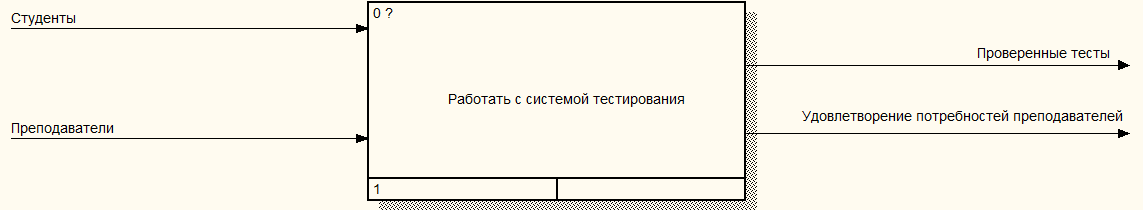
\includegraphics[width=\textwidth, center]{../img/idef3/Context.png}
    \caption{Контекстная диаграмма верхнего уровня}
\end{figure}

Данная диаграмма отображает наиболее общий вид модели системы тестирования.

\subsubsection{Работать с системой тестирования}
\begin{figure}[H]
    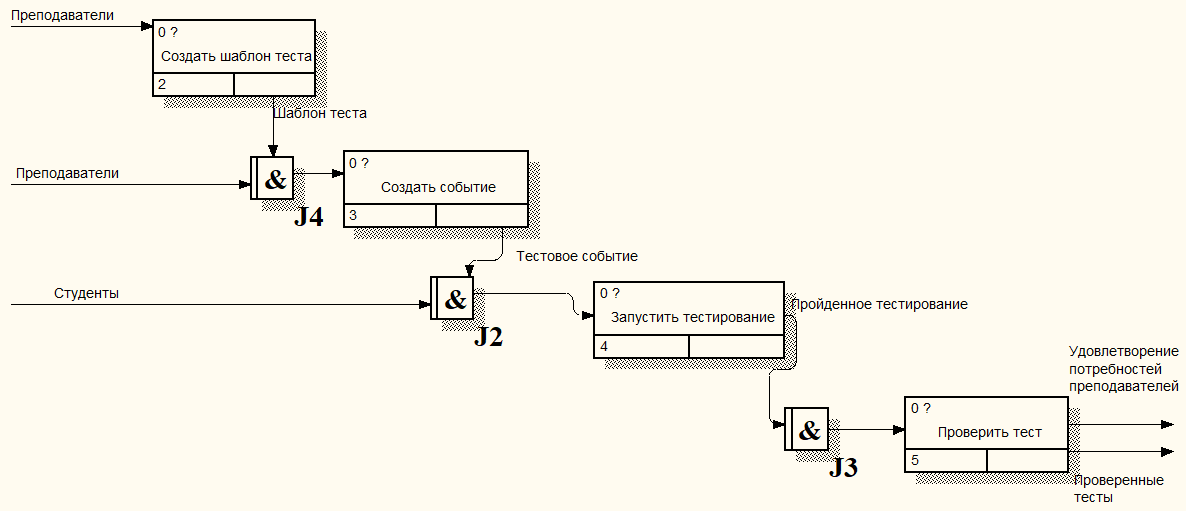
\includegraphics[width=\textwidth, center]{../img/idef3/ContextDecompose.png}
    \caption{Работать с системой тестирования}
\end{figure}

Преподаватели сначала создают шаблон теста, потом создают на основе этого шаблона
тестовое событие, которое запускают и проходят студенты, после чего пройденное 
тестирование проверяется системой на корректность, и результат проверки становится
доступен для студента, прошедшего тестирование и преподавателей.

\subsubsection{Создать шаблон теста}
\begin{figure}[H]
    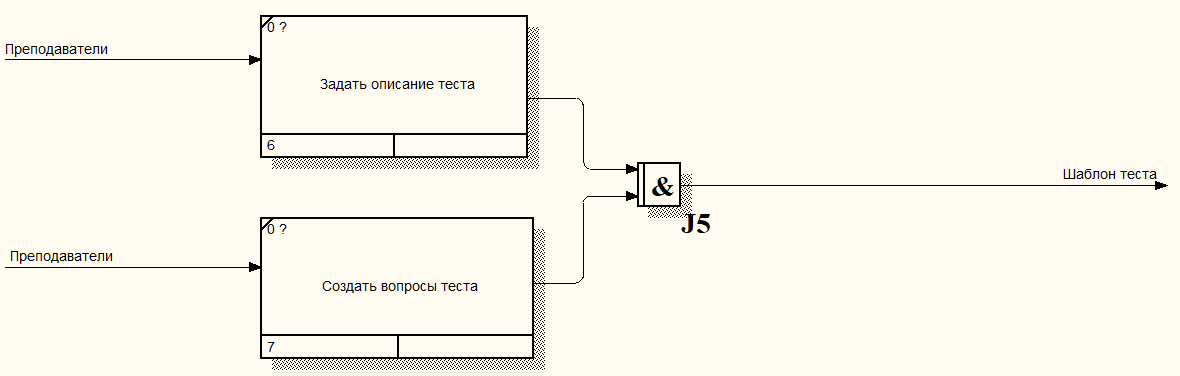
\includegraphics[width=\textwidth, center]{../img/idef3/CreateTestTemplate.png}
    \caption{Создать шаблон теста}
\end{figure}

Преподаватели задают описание теста и формируют вопросы теста, в результате чего
получает шаблон теста.

\subsubsection{Создать событие}
\begin{figure}[H]
    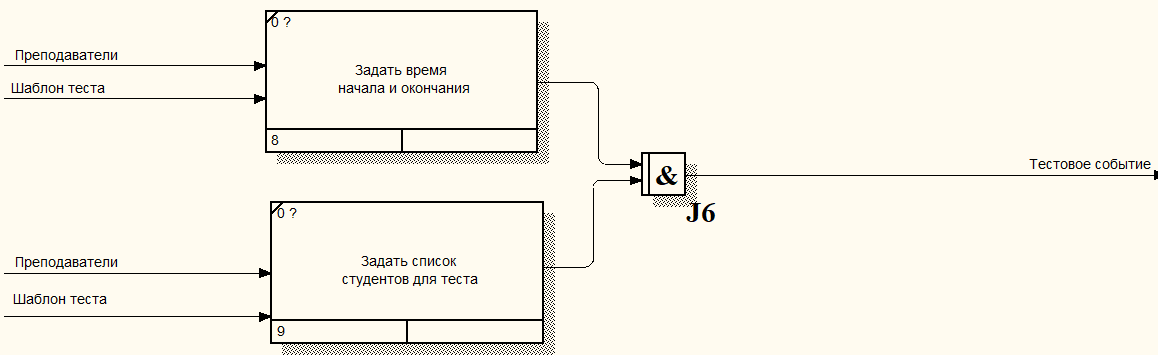
\includegraphics[width=\textwidth, center]{../img/idef3/CreateTestInstance.png}
    \caption{Создать событие}
\end{figure}

На основе шаблона теста преподаватель создает тестовое событие, для которого указывает
время начала и окончания и список студентов, которым необходимо принять участие
в этом событии.

\subsubsection{Запустить тестирование}
\begin{figure}[H]
    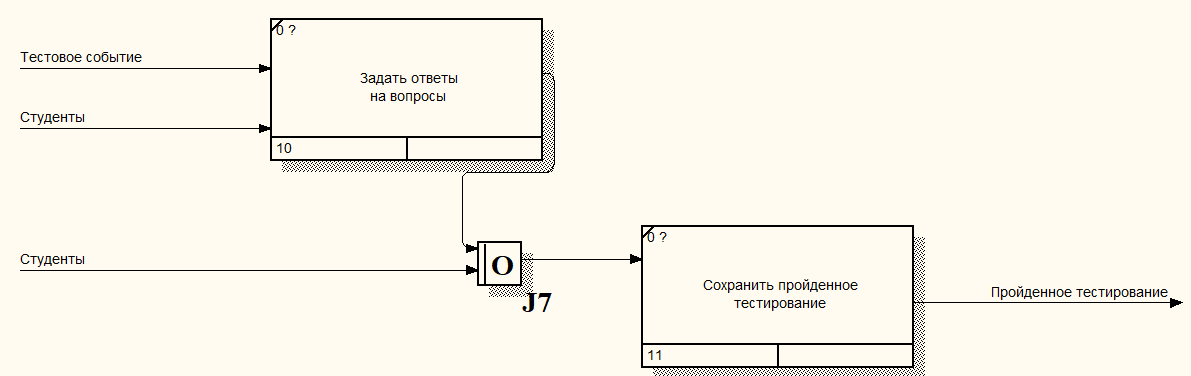
\includegraphics[width=\textwidth, center]{../img/idef3/RunTest.png}
    \caption{Запустить тестирование}
\end{figure}

Студент запускает выбранное тестовое событие и отвечает на вопросы теста,
если знает на них ответы. По завершении тестирования все ответы студента сохраняются.

\subsubsection{Проверить тестирование}
\begin{figure}[H]
    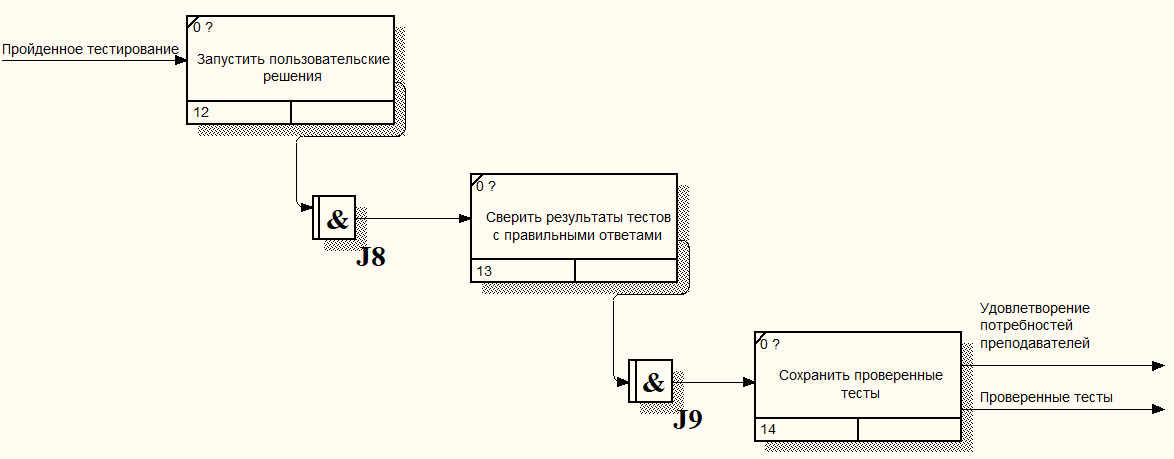
\includegraphics[width=\textwidth, center]{../img/idef3/ValidateTest.png}
    \caption{Проверить тестирование}
\end{figure}

После завершения тестирования система запускает код решений студента, получает
результаты работы алгоритмов и сравнивает их с правильными ответами на соответствующие вопросы.
После проверки результаты сохраняются и становятся доступны преподавателям и студенту,
проходившему тестирование.

\subsection{OSTN диаграмма}
\begin{figure}[H]
    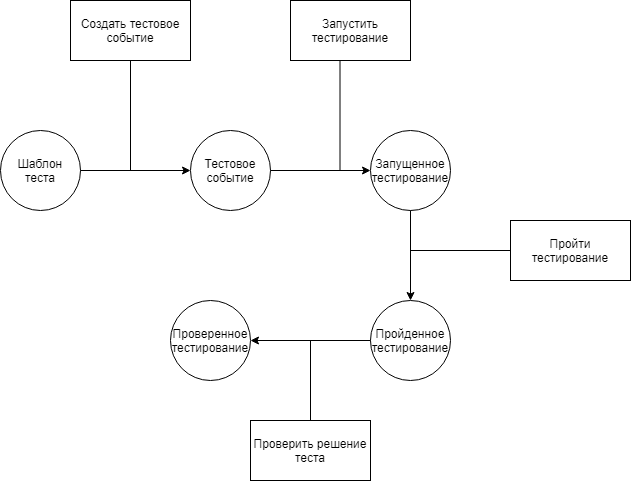
\includegraphics[width=\textwidth, center]{../img/OSTN.png}
    \caption{OSTN диаграмма}
\end{figure}

В системе не существует какого-то одного объекта, который подвергается изменениям.
Поэтому на данной диаграмме отображены основные объекты, которые присутствуют в
системе и образуются на различных этапах взаимодействия с ней.

Существуют следующие объекты:
\begin{enumerate}
    \item Шаблон теста
    \item Тестовое событие
    \item Запущенное тестирование
    \item Пройденное тестирование
    \item Проверенное тестирование
\end{enumerate}

Переходы:
\begin{enumerate}
    \item Шаблон теста -> Тестовое событие (событие создается на основе шаблона
    и имеет список назначенных на него студентов)
    \item Тестовое событие -> Запущенное тестирование (назначенный на событие студент
    может запустить его и начать проходить тестирование)
    \item Запущенное тестирование -> Пройденное тестирование (когда студент заканчивает
    прохождение тестирования, то оно становится пройденным, и его результаты сохраняются)
    \item Пройденное тестирование -> Проверенное тестирование (После прохождение тестирования
    система проверяет его и сохраняет результаты проверки)
\end{enumerate}


\subsection{DFD диаграммы}
\begin{figure}[H]
    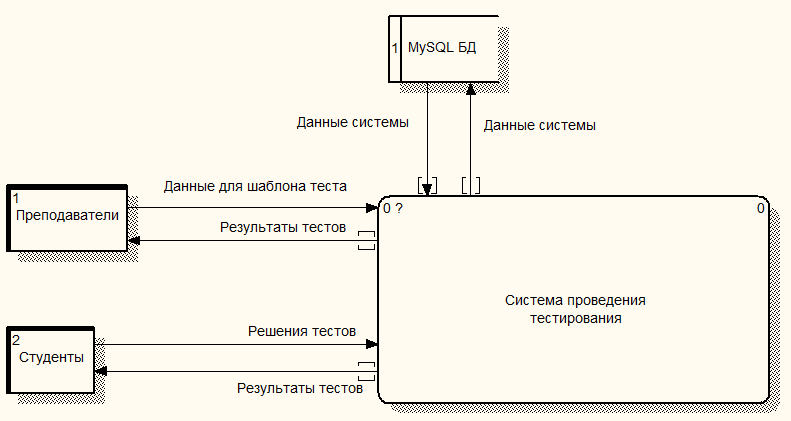
\includegraphics[width=\textwidth, center]{../img/dfd/context.png}
    \caption{Контекстная диаграмма верхнего уровня}
\end{figure}

Данная диаграмма в наиболее общем виде отображает потоки данных в автоматизированной
системе тестирования. Преподаватели создают шаблоны тестов и назначают тесты студентам
для прохождения. Студенты представляют свои решения на тестовые задания, после чего
система проверяет их, сохраняет результаты в базе данных и предоставляет студентам
и преподавателям возможность ознакомиться с результатами.

\textit{Потоки данных:}
\begin{enumerate}
    \item Данные для шаблона теста
    \item Данные системы
    \item Решения тестовое
    \item Результаты тестов
\end{enumerate}

\textit{Процесс (система)} - система проведения тестирования

\textit{Накопители данных} - MySQL база данных

\textit{Внешние сущности} - Студенты и преподаватели

\subsubsection{Система проведения тестирования}
\begin{figure}[H]
    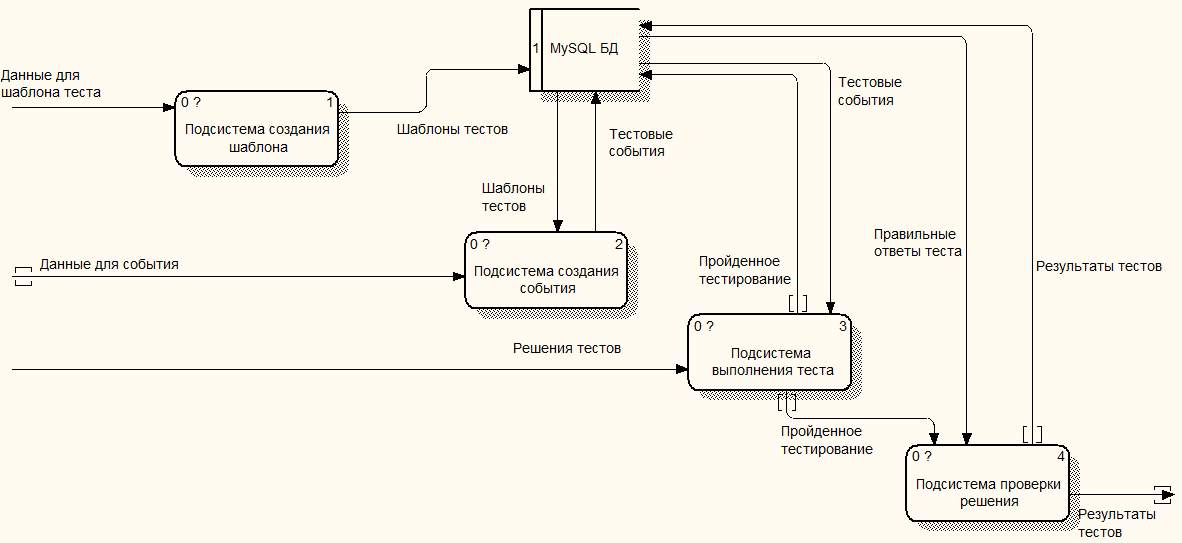
\includegraphics[width=\textwidth, center]{../img/dfd/ContextDecompose.png}
    \caption{Система проведения тестирования}
\end{figure}

Получив данные о шаблоне теста, подсистема создания шаблона создает шаблон и сохраняет
его и связанные с ним сущности в базе данных.

Подсистема создания события при
получении данных для события загружает из базы данных тестовый шаблон, создает событие
и также сохраняет его в базе данных.

Подсистема выполнения теста загружает тестовые события из базы данных, получает решения
задач от пользователя и сохраняет их в базе данных, после чего передает эти данные
подсистеме проверки решений, которая сверяет правильность результатов и сохраняет их в базе
данных.

\textit{Потоки данных:}
\begin{enumerate}
    \item Данные для шаблона теста
    \item Шаблоны тестов
    \item Тестовые события
    \item Пройденное тестирование
    \item Правильные ответы теста
    \item Результаты тестов
\end{enumerate}

\textit{Подсистемы:}
\begin{enumerate}
    \item Подсистема создания шаблона
    \item Подсистема создания события
    \item Подсистема выполнения теста
    \item Подсистема проверки решения
\end{enumerate}

\textit{Накопители данных} - MySQL база данных


\subsubsection{Подсистема создания шаблона}
\begin{figure}[H]
    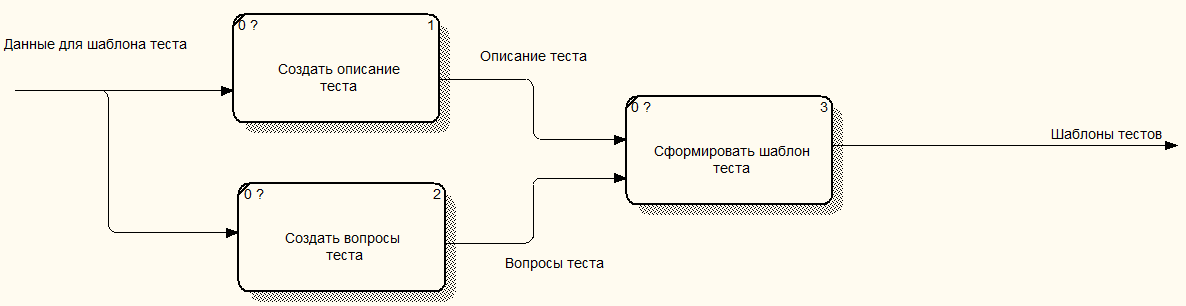
\includegraphics[width=\textwidth, center]{../img/dfd/Subsystem_Template.png}
    \caption{Подсистема создания шаблона}
\end{figure}

Подсистема создания шаблона получает на вход данные шаблона, формирует описание теста
и создает тестовые вопросы и возвращает сформированный тестовый шаблон.

\textit{Потоки данных:}
\begin{enumerate}
    \item Данные для шаблона теста
    \item Описание теста
    \item Вопросы теста
    \item Шаблоны тестов
\end{enumerate}


\textit{Процессы}
\begin{enumerate}
    \item Создать описание теста
    \item Создать вопросы теста
    \item Сформировать шаблон теста
\end{enumerate}


\subsubsection{Подсистема создания события}
\begin{figure}[H]
    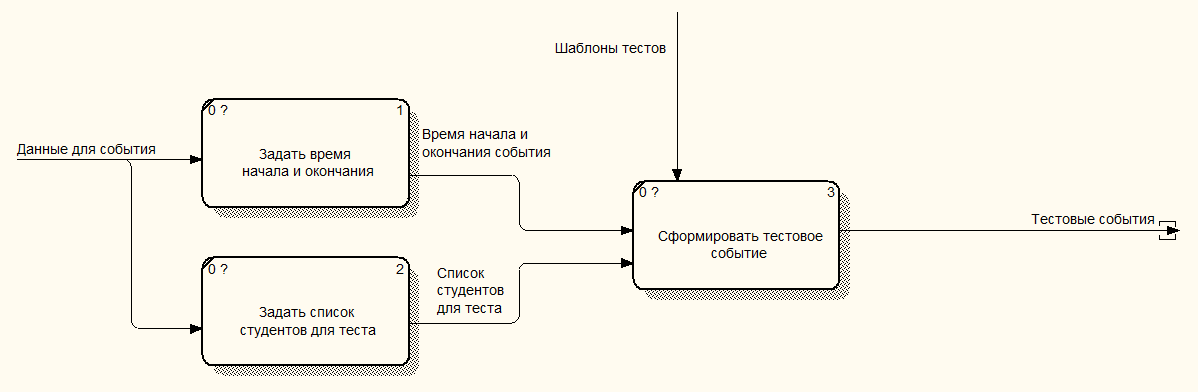
\includegraphics[width=\textwidth, center]{../img/dfd/Subsystem_Instance.png}
    \caption{Подсистема создания события}
\end{figure}

Подсистема создания события получает на вход данные для события, формирует время
начала и окончания события, список назначенных на тестирование студентов и
возвращает сформированное тестовое событие.


\textit{Потоки данных:}
\begin{enumerate}
    \item Данные для события
    \item Время начала и окончания события
    \item Список студентов для теста
    \item Тестовые события
\end{enumerate}


\textit{Процессы}
\begin{enumerate}
    \item Задать время начала и окончания
    \item Задать список студентов для теста
    \item Сформировать тестовое событие
\end{enumerate}


\subsubsection{Подсистема выполнения теста}
\begin{figure}[H]
    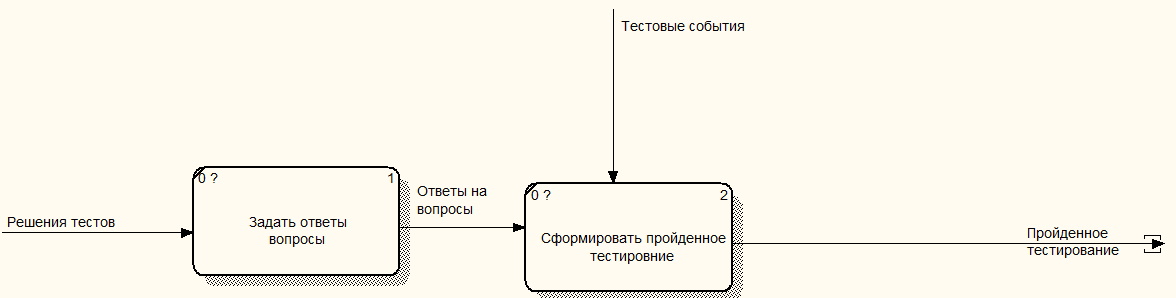
\includegraphics[width=\textwidth, center]{../img/dfd/Subsystem_Runner.png}
    \caption{Подсистема выполнения теста}
\end{figure}

Подсистема выполнения теста на вход получает решения тестов и тестовые событие
и формирует из этих данных пройденное тестирование.

\textit{Потоки данных:}
\begin{enumerate}
    \item Решения тестов
    \item Ответы на вопросы
    \item Тестовые события
    \item Пройденное тестирование
\end{enumerate}

\textit{Процессы}
\begin{enumerate}
    \item Задать ответы на вопросы
    \item Сформировать пройденное тестирование
\end{enumerate}


\subsubsection{Подсистема проверки решения}
\begin{figure}[H]
    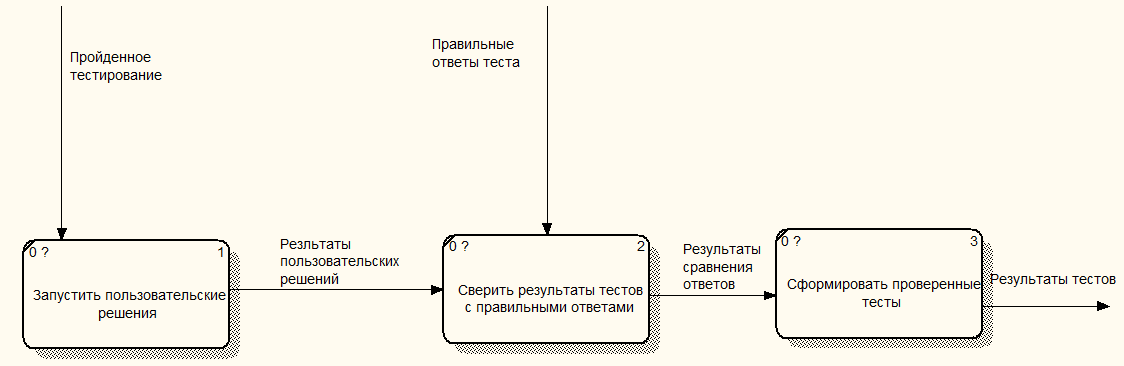
\includegraphics[width=\textwidth, center]{../img/dfd/Subsystem_Validator.png}
    \caption{Подсистема проверки решения}
\end{figure}

Подсистема проверки решения на вход получает пройденное тестирование и правильные
ответы теста, запускает пользовательские решения и сравнивает результаты, после
чего формирует проверенные тесты и возвращает результаты.

\textit{Потоки данных:}
\begin{enumerate}
    \item Пройденное тестирование
    \item Результаты пользовательских решений
    \item Результаты сравнения ответов
    \item Результаты тестов
\end{enumerate}

\textit{Процессы}
\begin{enumerate}
    \item Запустить пользовательские решения
    \item Сверить результаты тестов с правильными ответами
    \item Сформировать проверенные тесты
\end{enumerate}